\chapter{Обзор предметной области}
В данной обзорной главе будет представлена предметная область биоинформатики, введено понятие экспрессии генов, рассмотрены существующие решения для анализа экспрессии генов, а также перечислен ряд технологий, которые используются или могут быть использованы для создания инструментов анализа экспрессии генов.
\section{Биоинформатика}
\textbf{Биоинформатика} --- наука, объединяющая в себе методы прикладной математики, статистики, информатики для создания новых методов и алгоритмов для анализа разного рода биологических данных.

Биоинформатика занимается биохимией, биофизикой, экологией и многими другими областями биологии. Однако фокус в данной работе будет сосредоточен на конкретную задачу биоинформатики --- анализ экспрессии генов.

\subsection{Анализ экспрессии генов}
\textbf{Экспрессия генов} --- процесс преобразования наследственной информации от гена (в виде последовательности нуклеотидов ДНК) в функциональный продукт (РНК или белок).

Анализ экспрессии генов позволяет выяснить, как ведет себя каждый отдельный ген в разных условиях, тканях или организмах.

Экспрессия гена в образце характеризуется вещественным числом, которое также можно назвать некоторой мерой активности гена в данных условиях.

\subsection{Используемые методы}
Как было сказано ранее, биоинформатика использует в себе математику, информатику и статистику. Соответственно, задача анализа экспрессии генов сводится к исследованию путем статистических методов и алгоритмов числовой двумерной матрицы, где в виде вещественных чисел демонстрируется активность каждого гена в каждом образце. Пример такой матрицы можно увидеть в таблице~\ref{matrix}.

\begin{table}[!h]
\caption{Срез матрицы GSE14308. Строки матрицы соответствуют генам, столбцы --- образцам.}\label{matrix}
\centering
\begin{tabu} to \textwidth {| r |*{5}{ X[c] |}}
\hline
       & GSM357839	& GSM357841	& GSM357842	& GSM357843	& GSM357844	 \\\hline
Rps29	 & 16.32	    & 16.30	    & 16.25	    & 16.32	    & 16.30	     \\\hline
Rpl13a & 16.27	    & 16.23	    & 16.32	    & 16.30	    & 16.27	     \\\hline
Rps3a1 & 16.23	    & 16.19	    & 16.30	    & 16.25	    & 16.25	     \\\hline
Rpl38	 & 16.21	    & 16.25	    & 16.27	    & 16.27	    & 16.21	     \\\hline
Tmsb4x & 16.30	    & 16.32	    & 16.23	    & 16.21	    & 16.32	     \\\hline
\end{tabu}
\end{table}

Одним из первоочередных методов, применяемых для анализа экспрессии, является \textit{визуальный анализ}. Числовая матрица представляется в виде \textit{тепловой карты}, где цветом показана активность каждого гена. 

На рисунке~\ref{matrixvis} можно увидеть визуализацию матрицы экспрессии из таблицы~\ref{matrix} в виде тепловой карты.
\begin{figure}[h]
  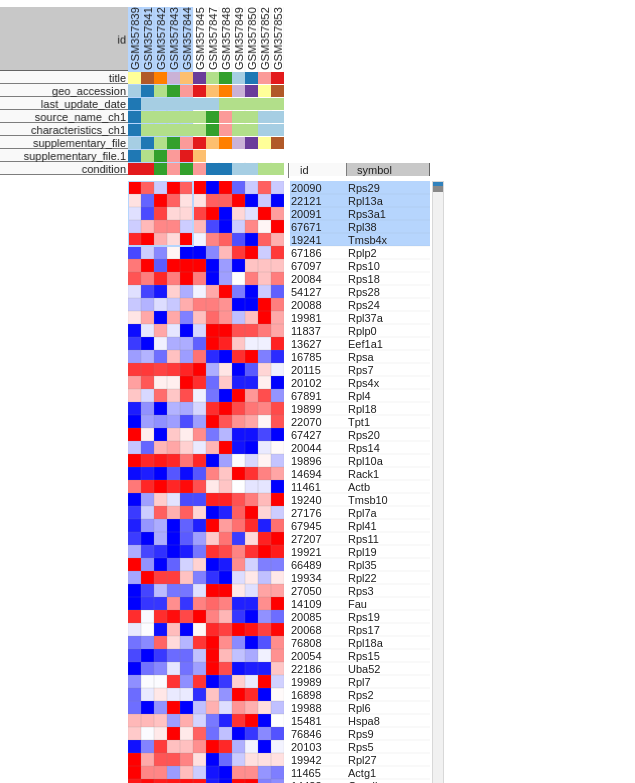
\includegraphics[scale=0.5]{heatmap14308.png}
  \caption{Визуализация матрицы GSE14308 в виде тепловой карты в веб-приложении Morpheus}
  \label{matrixvis}
\end{figure}


Также к основным методам анализа относятся:
\begin{itemize}
\item кластеризация:\begin{itemize}
\item иерархическая: метод упорядования данных таким образом, чтобы их можно было визуализировать в виде дерева (дендрограммы);
\item вероятностная: метод разбиения данных на несколько групп (кластеров);\end{itemize}
\item дифференциальная экспрессия: метод, позволяющий сравнивать поведение генов в разных условиях и искать закономерности;
\item метод главных компонент: метод для уменьшения размерности данных с наименьшей потерей информации. 
\end{itemize}

\section{Существующие решения для анализа экспрессии генов}
\subsection{R/Bioconductor}
\textbf{R} --- язык программирования для статистического анализа данных и работы с графикой~\cite{rproject}.

\textbf{Bioconductor} --- библиотека, содержащая в себе множество реализаций биоинформатических алгоритмов и методов обработки биологических данных на \emph{R}. Она постоянно обновляется, пополняется новыми библиотеками, модерируется сообществом~\cite{biobase}. \emph{R} и \emph{Bioconductor} очень популярны в биоинформатической среде ввиду предоставляемых возможностей.

Однако для качественного и полноценного анализа с помощью этих инструментов, нужно иметь навыки программирования на \emph{R}, что весьма неудобно для исследователей биологических специальностей.

\subsubsection{Biobase и ExpressionSet}
Необходимый минимум функций для работы с геномными данными содержится в \emph{R}-пакете \emph{Biobase}~\cite{biobase}.

Класс \texttt{ExpressionSet}~\cite{expressionset} также содержится в \emph{Biobase}. Он помогает представлять данные об экспрессии генов в удобном формате:
\begin{itemize}
\item \texttt{assayData} --- описание матрицы:\begin{itemize}
\item \texttt{features} --- количество генов;
\item \texttt{samples} --- количество образцов;
\item \texttt{exprs} --- числовая матрица экспрессии; \end{itemize}
\item \texttt{phenoData} --- аннотация к образцам:\begin{itemize}
\item \texttt{sampleNames} --- идентификаторы образцов;
\item \texttt{varLabels} --- названия характеристик;
\item \texttt{varMetadata} --- описание характеристик;
\item \texttt{pData} --- матрица характеристик;\end{itemize}
\item \texttt{featureData} --- аннотация к генам:\begin{itemize}
\item \texttt{featureNames} --- идентификаторы генов;
\item \texttt{fvarLabels} --- названия характеристик;
\item \texttt{fvarMetadata} --- описание характеристик;
\item \texttt{fData} --- матрица характеристик.\end{itemize}
\end{itemize}

Для доступа к каждому из элементов есть одноименная функция, что позволяет удобно взаимодействовать с экземплярами класса. Также многие из функций обработки данных в \emph{Bioconductor} и в \emph{Biobase} в частности завязаны на использование \texttt{ExpressionSet}.


\subsection{GENE-E}
\textbf{GENE-E} --- Платформа для анализа данных и визуального исследования данных, созданная на \emph{Java} и \emph{R}~\cite{genee}. Содержит в себе множество полезных для исследования инструментов: тепловые карты, кластеризацию, фильтрацию, построение графиков и т.д. Позволяет исследовать любые данные в виде матрицы. К тому же, содержит дополнительные инструменты для данных генетической экспрессии.

Недостатки:
\begin{itemize}
\item чтобы использовать, необходимо устанавливать на свой компьютер;
\item поддержка данного приложения прекратилась в связи с созданием \emph{morpheus.js}~\cite{morpheus};
\item не имеет открытого исходного кода, а только \emph{API} для взаимодействия и создания новых приложений на его основе.
\end{itemize}

\subsection{morpheus.js}
\textbf{Morpheus.js} --- веб-приложение для визуализации и анализа матриц от создателя \emph{GENE-E}~\cite{morpheus}. В отличие от предшественника, создано на \emph{JavaScript} и с открытым исходным кодом. Удобно для использования исследователями без навыков программирования и так же, как и \emph{GENE-E}, применимо к любым матрицам.

Недостатки:
\begin{itemize}
\item ограниченный набор функций, которых недостаточно для полноценного анализа;
\item для расширения биоинформатическими алгоритмами, не прибегая к дополнительным инструментам, требуется реализовывать их заново на \emph{JavaScript};
\end{itemize}

Далее будут описаны основные компоненты, классы и методы, реализованные в \emph{morpheus.js}, с которыми необходимо работать в случае расширения данного приложения.

\subsubsection{Чтение данных}
В \emph{morpheus.js} данные могут быть загружены из файла одним из следующих путей:
\begin{itemize}
\item Из компьютера;
\item По \emph{URL}-ссылке;
\item Из \emph{Dropbox}.
\end{itemize}

Допустимые форматы загружаемых файлов:
\begin{itemize}
\item \emph{txt}-файл с \emph{tab}-разделителями;
\item \emph{Excel}-таблица;
\item \emph{Mutation Annotation Format} (\emph{MAF})~\cite{maf};
\item \emph{Gene Cluster Text} (\emph{GCT})~\cite{gct};
\item \emph{Gene Matrix Transposed} (\emph{GMT})~\cite{gmt}.
\end{itemize}

Для каждого формата файла в исходном коде morpheus.js присутствует соответствующий обработчик данных.

Также, \emph{morpheus.js} предлагает набор предзагруженных данных из базы \emph{The Cancer Genome Atlas} (\emph{TCGA})~\cite{tcga}.

\subsubsection{Класс Dataset}
Одним из ключевых классов всего веб-приложения является класс \texttt{Dataset}. В каждом экземпляре этого класса хранится вся необходимая информация о данных, в которую входят:

\begin{itemize}
\item числовая матрица, характеризующая уровень экспрессии всех генов во всех образцах;
\item количество строк и столбцов в матрице;
\item аннотация к образцам, например:\begin{itemize}
\item пол, возраст, контактную информацию испытуемых, если образцы были взяты с людей;
\item есть или нет инфекция в данном образце;
    \item способ лечения;
    \item  контакты ответственного за взятие данного образца и пр.;\end{itemize}
\item аннотация к генам, например:\begin{itemize}
    \item идентификатор гена в том или ином стандарте;
    \item числовые характеристики гена (средний уровень экспрессии по образцам, номер кластера) и пр.\end{itemize}
\end{itemize}

Аннотация реализована в классе \texttt{MetadataModel}, который представляет собой не что иное, как набор именованных векторов с характеристиками. В каждом векторе хранятся:

\begin{itemize}
\item название;
\item формат (строка, число);
\item массив значений.
\end{itemize}

Для векторов так же предусмотрены утилиты для визуализации. Так, например, есть возможность показать аннотацию в виде текста и/или цветом, что удобно для категориальных характеристик. 

\subsubsection{Класс SlicedDatasetView}
Чаще всего во время работы программы экземпляры класса \texttt{Dataset} становятся обернуты в оболочку из \texttt{SlicedDatasetView}. Этот дополнительный класс дает возможность не пересоздавать каждый раз \texttt{Dataset}, а просто добавляет к данным информацию о том, какие индексы строк и столбцов выбраны и используются в данный момент и в каком порядке.

\subsubsection{Класс HeatMap}
Данный класс предназначен для визуализации данных, обернутых в класс \texttt{Dataset} или \texttt{SlicedDatasetView}. Он дает возможность выбирать, какая аннотация будет представлена на экране, цветовой код, выбирать строки и столбцы, с которыми будут работать те или иные инструменты.

\subsubsection{Класс DatasetUtil}
Класс \texttt{DatasetUtil} содержит в себе утилиты для обработки и чтения данных в \texttt{Dataset}:\begin{itemize}
\item обработка входных файлов с данными и отправка их на соответствующий класс чтения в зависимости от формата;
\item поиск по данным;
\item преобразование данных в \emph{JSON} и обратно.
\end{itemize}

\subsubsection{Реализованные методы}
В \emph{morpheus.js} имеются реализации следующих методов обработки и анализа данных:

\begin{itemize}
\item \texttt{Adjust} --- инструмент для корректировки данных:\begin{itemize}
    \item $\log_{2}$;
    \item $\log_{2}^{-1}$;
    \item Квантиль-нормализация;
    \item Z-тест;
    \item Устойчивый Z-тест;\end{itemize}
\item \texttt{Collapse} --- инструмент, позволяющий агрегировать строки или столбцы с одинаковыми значениями с помощью функции: $\min$, $\max$, $mean$, $median$, $sum$, максимум 25-го и 75-го перцентилей;
\item \texttt{CalculatedAnnotation} --- добавление вычисленной аннотации для строк или столбцов;
\item \texttt{Similarity Matrix} --- построение матрицы соответствия строк или столбцов друг другу;
\item \texttt{Transpose} --- транспонирование матрицы;
\item \texttt{t-SNE} --- реализация алгоритма снижения размерности;
\item \texttt{ChartTool} --- построение графиков.
\end{itemize}

Также присутствуют фильтрация и сортировка.

\subsection{ProjectX}
\textbf{ProjectX} --- веб-приложение, созданное в рамках выпускной квалификационной работы~\cite{projectx}, которое соединяло в себе возможности, предоставляемые \emph{API} \emph{GENE-E} и методы из библиотеки \emph{Bioconductor} с помощью \emph{OpenCPU}. Реализовано было данное приложение во фреймворке \emph{Django}. Преимуществом данного приложения перед \emph{GENE-E} была вопроизводимость исследований (на каждом этапе пользователь мог скачать исполняемый \emph{R}-код, эквивалентный коду, выполненному в сервисе), также он содержал в себе большее число методов анализа и обработки данных.

Недостатки:
\begin{itemize}
\item проект использовал в своей базе приложение, которое больше не поддерживается разработчиками;
\item работа над проектом была завершена до того, как у него появились пользователи, так что оно осталось невостребованным.
\end{itemize}

\section{Использование R в веб-разработке}
Как было сказано ранее, \emph{R} удобно использовать для статистического анализа данных. Но чтобы использовать методы \emph{R} в веб-приложениях, возникает необходимость в дополнительных технологиях для интеграции инструментов веб-разработки и \emph{R}.

\subsection{Shiny}
\textbf{Shiny} --- фреймворк для создания веб-приложений, используя только язык \emph{R}~\cite{shiny}.
\subsection{OpenCPU}
\textbf{HTTP} (\emph{HyperText Transfer Protocol}) ---  протокол прикладного уровня передачи данных на основе технологии <<клиент-сервер>>~\cite{http}.

\textbf{HTTP API} - набор процедур и функций, вызов которых и возвращение их результа осуществляется посредством протокола \emph{HTTP}.

\textbf{RPC} (\emph{Remote Procedure Call}) --- класс технологий, позволяющих компьютерным программам вызывать функции или процедуры в другом адресном пространстве.

\textbf{Веб-сервер} --- сервер, принимающий \emph{HTTP}-запросы от клиентов, обычно веб-браузеров, и выдающий им \emph{HTTP}-ответы.

\textbf{OpenCPU} --- система для встроенных научных вычислений и воспроизводимых исследований, предоставляющая \emph{HTTP API} для вызова R-функций и взаимодействия с R-объектами с помощью \texttt{POST} и \texttt{GET} запросов~\cite{opencpu}.

\subsubsection{OpenCPU-сервер}
\emph{OpenCPU}-сервер можно запустить одним из следующих способов:
\begin{itemize}
\item однопользовательский сервер: сервер запускается из активной \emph{R}-сессии и предназначен в основном для разработки и локального использования. Такой сервер не поддерживает параллельных запросов, так как \emph{R}-сессии работают в одном потоке;
\item облачный сервер: этот сервер можно запустить на \emph{Ubuntu 16.04} и выше. Запуск и настройка облачного сервера осуществляется с помощью \emph{Apache} или \emph{Nginx}. В отличие от однопользовательского сервера, здесь поддерживаются параллельные запросы и настройка безопасности.
\end{itemize}

Однопользовательский сервер в большинстве случаев работает значительно быстрее, чем облачный, так как последний управляется с помощью \emph{rApache}~\cite{rapache}, что добавляет удобства в использовании, но замедляет доступ к серверу. Первым же можно пользоваться как многопользовательским, используя несколько экземпляров сервера, доступ к которым осуществляется с помощью \emph{Apache} и балансировщика, который тот предоставляет.

\subsubsection{OpenCPU API}
Входной точкой \emph{API} является \texttt{/ocpu/}.
\texttt{GET}-запрос используется для получения некоторого ресурса, а \texttt{POST}-запрос используется для \emph{RPC}. На таблице~\ref{ocpu_api} можно увидеть более подробное описание запросов.

\begin{table}[!h]
  \small
\caption{Запросы к \emph{OpenCPU}-серверу, их аргументы и действия}\label{ocpu_api}
\centering
\begin{tabu} to \textwidth {| l | L | K | X |}
  \hline
Запрос        & Действие          & Аргументы                    & Пример                                 \\\hline 
\texttt{GET}  & посмотреть объект & формат представления объекта & GET /ocpu/library/MASS/R/cats/json     \\\hline
\texttt{POST} & вызвать функцию   & аргументы функции            & POST /ocpu/library/stats/R/rnorm       \\\hline
\texttt{GET}  & прочитать файл    & -                            & GET /ocpu/library/MASS/NEWS            \\\hline
\texttt{POST} & запустить скрипт  & аргументы запуска скрипта    & POST /ocpu/library/MASS?scripts/ch01.R \\\hline
\end{tabu}
\end{table}

На \emph{OpenCPU}-сервере могут быть доступны:
\begin{itemize}
\item библиотеки и содержащиеся в них пакеты: \texttt{/ocpu/library/{pkgname}/};
\item пакеты из \emph{git}-репозиториев: \texttt{/ocpu/apps/{gituser}/{reponame}/};
\item пакеты, установленные в домашней директории \emph{Linux}-пользователя: \texttt{/ocpu/user/{username}/library/{pkgname}/};
\item временные сессии, содержащие вывод от запуска функции или скрипта: \texttt{/ocpu/tmp/{key}/}.
\end{itemize}

\subsubsection{Opencpu.js}
Так как зачастую \emph{OpenCPU} используется разработчиками для использования \emph{R} в веб-приложениях для анализа и визуализации данных, для удобной интеграции \emph{JavaScript} и \emph{R} существует библиотека \textit{opencpu.js}, которая реалазует \emph{RPC}-вызовы по принципу \emph{Asynchronous JavaScript and XML} (\emph{Ajax}~\cite{ajax}). Таким образом запросы обрабатываются в фоновом режиме, тем самым не замедляя работу графического интерфейса и вычислений, осуществляемых на стороне клиента.

В данной библиотеке реализован класс \texttt{Session}, содержащий в себе ключ сессии, адреса на ссылки, файлы и переменные, существующие внутри сессии.

Для подключения к \emph{R}-пакету на \emph{OpenCPU}-сервере удобно использовать код, представленный на листинге~\ref{connect}. Для успешного подключения \emph{R}-пакет должен быть предварительно установлен на \emph{host}-машину, на которой располагается сервер. 

\begin{lstlisting}[float=!h,caption={Подключение к \emph{R}-пакету},label={connect}]
  ocpu.seturl("//hostname/ocpu/library/{pkgname}/R");
\end{lstlisting}
После этого можно вызывать и запускать функции, содержащиеся в данном \emph{R}-пакете, например, как в листинге~\ref{call.example}.

\begin{lstlisting}[float=!h,caption={Шаблон вызова \emph{R}-функции из \emph{JavaScript}},label={call.example},language=JavaScript]
  var req = ocpu.rpc("function.name", arguments, callback(session) {
    \\ Handling result
  });
\end{lstlisting}

\section{Инфраструктура}
\subsection{Docker}
\textbf{Docker} --- программное обеспечение для автоматизации запуска и внедрения приложений внутри контейнеров~\cite{docker}.

Для дальнейшего описания данного инструмента введем несколько определений.

\textit{Образ} --- отдельный исполняемый пакет, включающий себя все необходимое для запуска единицы программного обеспечения, в том числе исходный код, библиотеки, переменные окружения, конфигурационные файлы. Зачастую образ построен на основе другого образа с дополнительной конфигураций. Образ компилируется по \textit{Dockerfile}, каждая команда в котором соответствует новому слою. При перекомпиляции обновляются только те слои, которые изменились. 

\textit{Контейнер} --- запущенный экземпляр образа. Контейнер обычно исполняется изолированно от окружения, имея доступ к файлам или портам хост-системы только при наличии соответствующей конфигурации.

В отличие от виртуальных машин, которые запускают гостевую операционную систему в каждом экземпляре, контейнеры могут разделять общее ядро, и вся информация, которая должна быть в контейнере, это исполняемый процесс и его зависимости. Исполняемые процессы из контейнеров работают как нативные процессы, и могут управляться по отдельности. 

Для контроля версий и хранения образов в открытом доступе используется \emph{Docker Hub}~\cite{dhub}. В этом хранилище можно как добавлять репозитории, управляемые вручную, так и поддерживать автоматические сборки (\textit{Automated Build}), которые привязаны к репозиториям на в популярных системах контроля версий: GitHub~\cite{github} и Bitbucket~\cite{bitbucket}.
\subsection{Apache}
\textbf{Apache HTTP Server Project} --- устойчивый, полностью открытый \emph{HTTP}-сервер~\cite{apache}.

\section{Форматы сериализации данных}
\subsection{JSON}
\textbf{JSON} --- текстовый формат представления данных, основанный на \emph{JavaScript}, который, среди прочих достоинств, легко читается человеком.

\emph{JSON}-текст представляет собой одну из следущих структур:\begin{itemize}
\item пара \textit{ключ}: \textit{значение}, где ключом может быть только регистрозависимая строка, а в качестве значения может выступата массив, число, строка, литералы или другой \emph{JSON}-объект;
\item набор значений.
\end{itemize}

\subsection{Protocol Buffers}
\textbf{Protocol Buffers (Protobuf)} --- гибкий, универсальный и автоматизированный механизм для сериализации структурированных данных~\cite{protobuf}.

Структура информации задается с помощью \texttt{*.proto}-файлов в форме сообщений (\texttt{message}).

\emph{ProtoBuf}-формат не является человекочитаемым, данные хранятся в двоичном формате. Для десериализации и дальнейшего чтения необходим соответствующий \texttt{*.proto}-файл. Файл с форматом компилируется соответствующим выбранному языку программирования компилятором, таким образом будет создан класс доступа к данным. С помощью этого класса уже можно сериализовать/десериализовать данные, получать данные с помощью \texttt{get}/\texttt{set}-методов и пр.

\section{Открытые источники данных экспрессии генов}
\subsection{Gene Expression Omnibus}
\textbf{Gene Expression Omnibus (GEO)} --- международный публичный репозиторий, агрегирующий и распространяющий различные формы геномных данных от исследовательского сообщества~\cite{geo}.

\emph{GEO} предоставляет устойчивую базу данных для эффективного хранения геномных данных, содержит их в качественно аннотированном формате и дает возможность удобно как добавлять новые данные для публикации, так и запрашивать интересующие данные для исследований.

В \emph{GEO} содержатся следующие типы и форматы данных:
\begin{itemize}
\item информация о платформе, на которой производилось секвенирование генов (\emph{Platform records}): \texttt{GPLxxx};
\item информация об образцах и условиях, в которых производились исследования этих образцов (\emph{Sample records}): \texttt{GSMxxx};
\item информация о непосредственно исследованиях, полученные данные и выводы (\emph{Series records}): \texttt{GSExxx}.
\item обработанная и подготовленная для дальнейшего статистического анализа \emph{GEO}-кураторами информация об исследованиях (\emph(DataSet records)): \texttt{GDSxxx}.
\end{itemize}

В библиотеке \emph{Bioconductor} есть \emph{R}-пакет \emph{GEOquery} для удобной загрузки данных из \emph{GEO}~\cite{geoquery}.
\subsection{The Cancer Genome Atlas}
\textbf{The Cancer Genome Atlas (TCGA)} --- проект, нацеленный на систематизацию данных о генетических мутациях, приводящих к возникновению рака. На данный момент участниками проекта отсеквенировано и проанализировано 33 вида рака~\cite{tcga}.

\section{Постановка задачи}
Рассмотрев существующие решения для анализа экспрессии генов и инструментов, которые могли бы пригодиться для будущих решений, можно сформулировать цель и основные задачи данной работы

\subsection{Цель работы}
Целью работы является создание веб-приложения, интегрирующего существующие возможности веб-приложения \emph{morpheus.js} и методы анализа, реализованные в \emph{Bioconductor}.

\subsection{Основные задачи}
Для достижения поставленной цели были сформулированы следующие задачи:
\begin{enumerate}
\item разработать способ взаимодействия между \emph{js}-клиентом и \emph{R} и встроить его в \emph{morpheus.js}, чтобы избежать реализации с нуля уже существующих алгоритмов;
\item реализовать графический интерфейс в \emph{js}-клиенте и серверную реализацию в \emph{R}-пакете;
\item соединить все составляющие в одном веб-приложении \emph{phantasus};
\item запустить веб-приложение в открытый доступ для исследователей.
\end{enumerate}

\subsection{Требования к веб-приложению phantasus}
\subsubsection{Доступность}
Необходимо, чтобы веб-приложение \emph{phantasus} было доступно для исследователей независимо от их местоположения и времени суток. Варианты действий:

\begin{enumerate}
\item сделать его доступным по определенному веб-адресу, и тогда пользователь сможет продолжать исследования из любой точки, где есть подключение к интернету;
\item предоставить возможность запускать приложение локально, например, с помощью \emph{Docker} или внутри \emph{R}.
\end{enumerate}

\subsubsection{Возможность дальнейшего расширения функционала}
Как уже было сказано выше, библиотека \emph{Bioconductor} постоянно обновляется и пополняется новыми алгоритмами, а исследователи находят новые методы для анализа экспрессии генов, так что необходимо не только реализовать дополнительные методы, но также отладить и описать алгоритм действий для добавления новых.

\chapterconclusion
В данной главе были введены понятия биоинформатики и анализа экспрессии генов, обозначена цель работы и задачи, выполнение которых необходимо для ее достижения, представлены существующие решения с их достоинствами и недостатками, а также перечислен ряд инструментов, которые могут быть использованы для решения поставленных задач работы.
